As described in \secref{intro_motivation}, deep networks suffer from early commitment.
However, the \emph{Gestalt} psychology \cite{ellis_source_1938, kohler_gestalt_1992, wagemans_century_2012, hamlyn_psychology_2017}, as well as the theory of natural intelligence \cite{von_der_malsburg_theory_2022} and work based on self-organising projection fibres \cite{bienenstock_neural_1987, lades_distortion_1993, wiskott_face_1996, fernandes_self-organization_2015} considers the principle of preventing early commitment as a core mechanism for the effectiveness of the human visual system.

The human brain can prevent early commitment \cite{marr_vision_2010} while still being an excellent image-processing system \cite{ellis_source_1938, kohler_gestalt_1992, wagemans_century_2012, hamlyn_psychology_2017}. 
Consequently, the neuroscientific literature is studied, and promising findings to implement a vision framework preventing early commitment are identified.
Thus, this chapter can be considered a survey of existing neuroscientific findings.
However, compared to the related work section, it contains more interpretations and introduces a unified vocabulary compatible with both fields, neuroscience and deep learning.

In the following, \secref{neuroscience_findings} presents important neuroscientific findings, describing lateral connections (\secref{neuroscience_findings_lateral_connections}), net fragments (\secref{neuroscience_findings_net_fragments}), the local learning principle (\secref{neuroscience_findings_local_learning_principle}), and projection fibres (\secref{neuroscience_findings_projection_fibres}).
Finally, \secref{biologial_inspiration_vision} describes how these biological findings could improve current systems.



\section{Neuroscientific Findings}\seclbl{neuroscience_findings}

\subsection{The Brain's Visual System}
\begin{figure}[h]
    \centering
    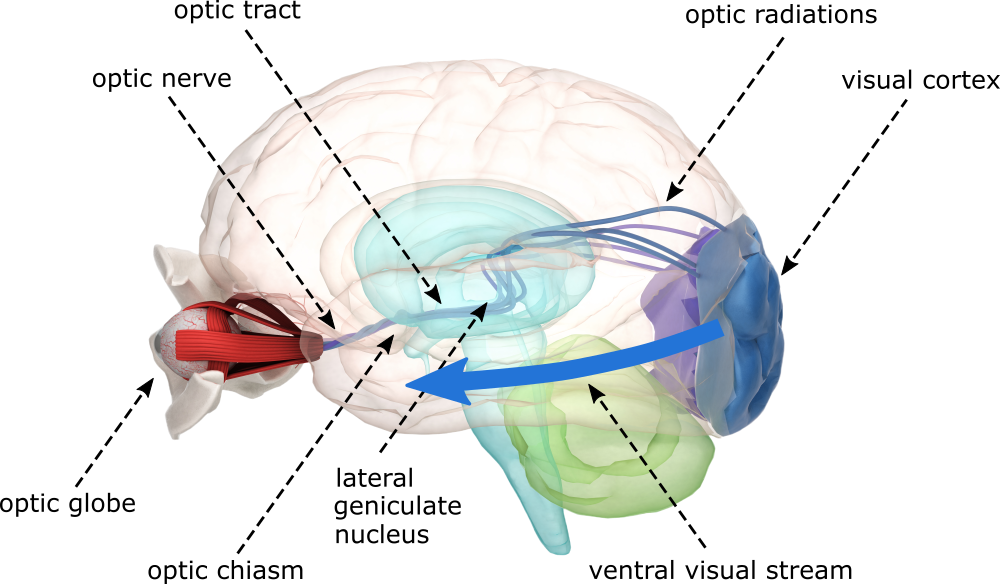
\includegraphics[width=0.99\textwidth]{Visual-System}
    \caption[Visualisation of the human's visual system]{Visualisation of the human's visual system. The image is from \citeay{fasoli_human_2023}.}
    \figlbl{visual_system}
\end{figure}
%
The visual system of humans is illustrated in \figref{visual_system}. The eyes are sensors that capture light waves and translate them into electrical pulses. These electrical signals travel through the human brain to the primary visual cortex \sidecite{tong_primary_2003, grill-spector_human_2004}, located at the back of the head.
Cells within the visual cortex fire spikes when specific visual stimuli appear within their receptive fields \cite{grill-spector_human_2004}. Thus, these cells can be considered filters that are excited if a known pattern is detected in the input data. 

The visual cortex detects patterns in visual data but does not draw conclusions from it. Instead, it forwards it as an information stream to other brain areas. In this thesis, especially the ventral visual stream \sidecite{goodale_separate_1992} is of importance, which forwards the detected patterns to the temporal cortex \sidecite{miyashita_inferior_1993, conway_organization_2018}, a brain region located behind the ears.
According to the two-stream hypothesis \cite{goodale_separate_1992}, the temporal cortex is responsible for object identification and recognition.
Thus, the visual cortex detects patterns that are compared with object prototypes stored in the temporal cortex.
A second stream, the dorsal stream \cite{goodale_separate_1992}, forwards the same data to the parietal cortex, a region on top of the head that predicts the object's spatial location relative to the viewer \sidecite{colby_space_1999}. However, this stream is of less importance in this thesis.

The brain leverages net fragments \sidecite{von_der_malsburg_concerning_2018}, lateral connections \sidecite{gilbert_lateral_1990, liang_interactions_2017, stettler_lateral_2002}, and projection fibres \sidecite{tanigawa_organization_2005} to process visual data. These fundamental elements of the brain serve as inspiration for the proposed framework and are introduced in the following.

\begin{figure}[h]
    \centering
    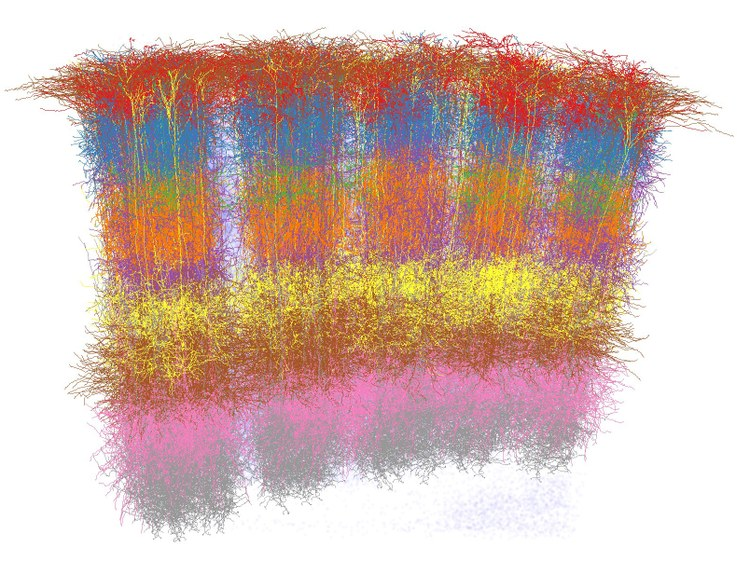
\includegraphics[width=0.99\textwidth]{cortical_columns}
    \caption[3D reconstruction of five neighbouring cortical columns]{3D reconstruction of five neighboring cortical columns of a rat. The image is from \citeay{oberlaender_beyond_2012}.}
    \figlbl{cortical_columns}
\end{figure}

\subsection{Lateral Connections}\seclbl{neuroscience_findings_lateral_connections}
The cerebral cortex forms the outer hull of the brain \sidecite{narr_relationships_2007} and encompasses several regions, including the previously mentioned visual and temporal cortex, as well as the ventral visual stream.
The cerebral cortex consists of many cylindrical arrangements of neurons called cortical columns \sidecite{mountcastle_columnar_1997}.
A 3D reconstruction of five cortical columns is shown in \figref{cortical_columns}, with different layers visualised by different colours.

Information in the cerebral cortex is propagated forward from one layer to the next and has inspired layer-wise processing in deep learning architectures \sidecite{prince_understanding_2023}.
However, a closer look at the human brain reveals that there are also connections between neurons within the same layer that process information locally \sidecite{gilbert_lateral_1990}.
These intra-layer connections are called \emph{lateral connections} \sidecite{liang_interactions_2017, stettler_lateral_2002} and are visualised in a simplified manner in \figref{lateral_connections} for a single neuron.
Notably, such a neuron not only establishes connections to neurons in the preceding and subsequent layers (marked in orange and green) but also lateral connections to neurons within its own layer (marked in red).

\begin{figure}[h]
    \centering
    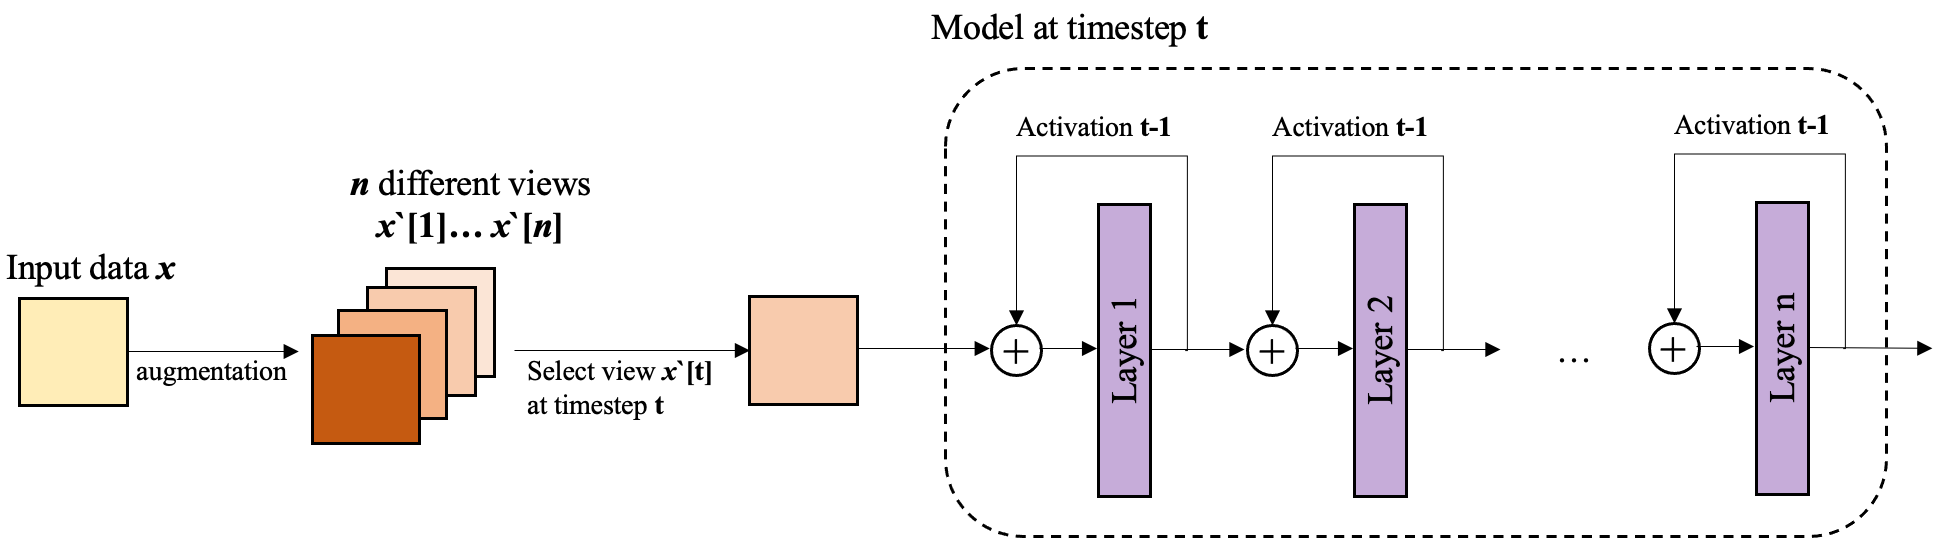
\includegraphics[width=0.99\textwidth]{lateral_connections}
    \caption[Lateral connections of a cell]{Visualisation of the connections of a single cell. The cell is connected to the previous layer (orange), the subsequent layer (green), and to neurons within the same layer (lateral connections, red).}
    \figlbl{lateral_connections}
\end{figure}

According to \sideciteay{von_der_malsburg_theory_2022}, these lateral connections are used for \emph{lateral support}. ``Lateral support'' means that neurons from the same layer support each other's activity:
Neurons from the preceding layer can activate the red cell in \figref{lateral_connections} through the orange connections.
However, inhibitory signals can suppress the activity \sidecite{coombs_specific_1955} of the red neuron before it can fire a spike to the subsequent layer via the green connections. The neuron can only transmit a spike to the subsequent layers if it ``survives'' an inhibition phase \sidecite{vogels_inhibitory_2011}, which is only possible if it receives sufficient lateral support \sidecite{stettler_lateral_2002} from laterally connected neurons.
Suppose the preceding layer activates several neurons within the same layer as the red neuron, and these activated neurons exhibit lateral connections. In that case, they can send spikes to each other, thereby providing mutual support. This allows them to maintain their action potential and remain active during the inhibition phase.

\subsection{Net Fragments}\seclbl{neuroscience_findings_net_fragments}
Lateral connections grow between cells that are often active together \sidecite{hebb_organization_1949}.
Since cells are often simultaneously active when representing the same pattern, lateral support is increased between groups of neurons representing frequently occurring patterns \cite{stettler_lateral_2002}. Such groups are called \emph{net fragments} \sidecite{von_der_malsburg_concerning_2018}.
All neurons within a net fragment support each other to remain active during an inhibition phase \sidecite{vogels_inhibitory_2011}. 
Thus, a layer with multiple net fragments can be considered a filter: While the previous layer might activate numerous cells, only the cells with sufficient lateral support remain active. Therefore, only learned patterns survive and send a spike to the next layer \cite{von_der_malsburg_concerning_2018}.

\subsubsection{Local Neighbourhood}
\begin{figure}[h]
    \centering
    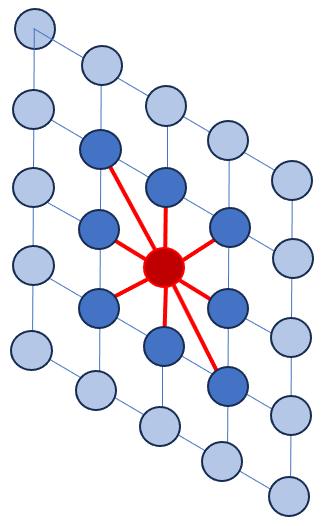
\includegraphics[width=0.4\textwidth]{local_neighbourhood2}
    \caption[Lateral connections limited to a local neighbourhood]{The lateral connections limited to a local neighbourhood.}
    \figlbl{local_neighbourhood2}
\end{figure}
Net fragments represent patterns that can be distinguished between local patterns, which are spatially limited to a local area, and global patterns, which extend over larger regions of the image and might encompass the entire image.
The number of possible patterns increases exponentially with the considered pattern size. Thus, local patterns occur more frequently.
To capture frequently occurring patterns, the visual cortex limits the range of lateral connections to a \emph{local neighbourhood} \sidecite{liang_interactions_2017, stettler_lateral_2002}.
Capturing global patterns would require exponentially more cells, and therefore, limiting the range of lateral connections to local neighbourhoods is crucial.
\figref{local_neighbourhood2} illustrates such limited lateral connections: The lateral connections from the red cell do not encompass the entire image but are only connected to cells in close proximity.

The size of the local neighbourhood in the human brain varies \sidecite{pessoa_understanding_2014}.
The primary visual cortex captures the input signal with a high variance and therefore has a strongly limited local neighbourhood size \sidecite{von_der_malsburg_concerning_2018}. The temporal cortex contains transformation-independent object representations and can afford larger neighbourhood sizes as fewer distinct global patterns exist \cite{von_der_malsburg_concerning_2018}.

\subsubsection{Hierarchy of Net Fragments}
A single cell is supported by its neighbouring cells, which, in turn, are supported by their neighbouring cells. Therefore, the support reaches much further than only the local neighbourhood \cite{von_der_malsburg_concerning_2018}, \sidecite{von_der_malsburg_theory_2022}.
As the processing progresses, increasing inhibition causes cells without sufficient support to be turned off. Turning off one cell can trigger a chain reaction of further turn-offs. Therefore, lateral support occurs not only between individual cells but also between many overlapping net fragments \cite{von_der_malsburg_theory_2022}.

Thus, the network consists of an overlay of net fragments, which can be interpreted as a larger net fragment, i.e. a multitude of cells supporting each other \cite{von_der_malsburg_theory_2022}.
The size of a net fragment cannot be defined; the smallest possible net fragment is a single cell with its local neighbourhood, while the largest net fragment can span all active cells that are laterally connected.
Furthermore, a single layer represents local and global features at the same time, whereby local features are stored in smaller net fragments and global features in larger net fragments \cite{von_der_malsburg_theory_2022}.
Thus, net fragments form a feature hierarchy within a layer \cite{von_der_malsburg_theory_2022}.

\subsubsection{Alternative Cells and Pathways}\seclbl{neuroscience_findings_alt_cells}
In a given spatial location, different patterns can occur.
However, the capacity of a net fragment is limited to represent a single pattern \sidecite{von_der_malsburg_theory_2022}.
For example, cell $A$ may often fire with cells $B$ and $C$ in close proximity, exhibiting a high mutual lateral support with these cells.
However, cells $B$ and $C$ might not fire together. Consequently, cell $A$ is involved in two distinct and mutually exclusive net fragments, once with cell $B$ and once with cell $C$.
To facilitate such coexistence between net fragments, \emph{alternative cells} are required \sidecite{von_der_malsburg_concerning_2018}. A copy of cell $A$ must exist that behaves similarly but has different synaptic connections, i.e. exhibits \emph{alternative pathways}.
The precise biological mechanism of how this is implemented is unclear; One hypothesis is that within a group of cells that initially have similar afferent connections, cells undergo divergent connectivity changes during training \sidecite{grossberg_competitive_1987}, resulting in cells specialising in different patterns. Thus, multiple similar feature cells could exist at the same spatial location and enable the formation of alternative and mutually exclusive net fragments.


\subsection{Projection Fibres}\seclbl{neuroscience_findings_projection_fibres}
\begin{figure}[h]
    \centering
    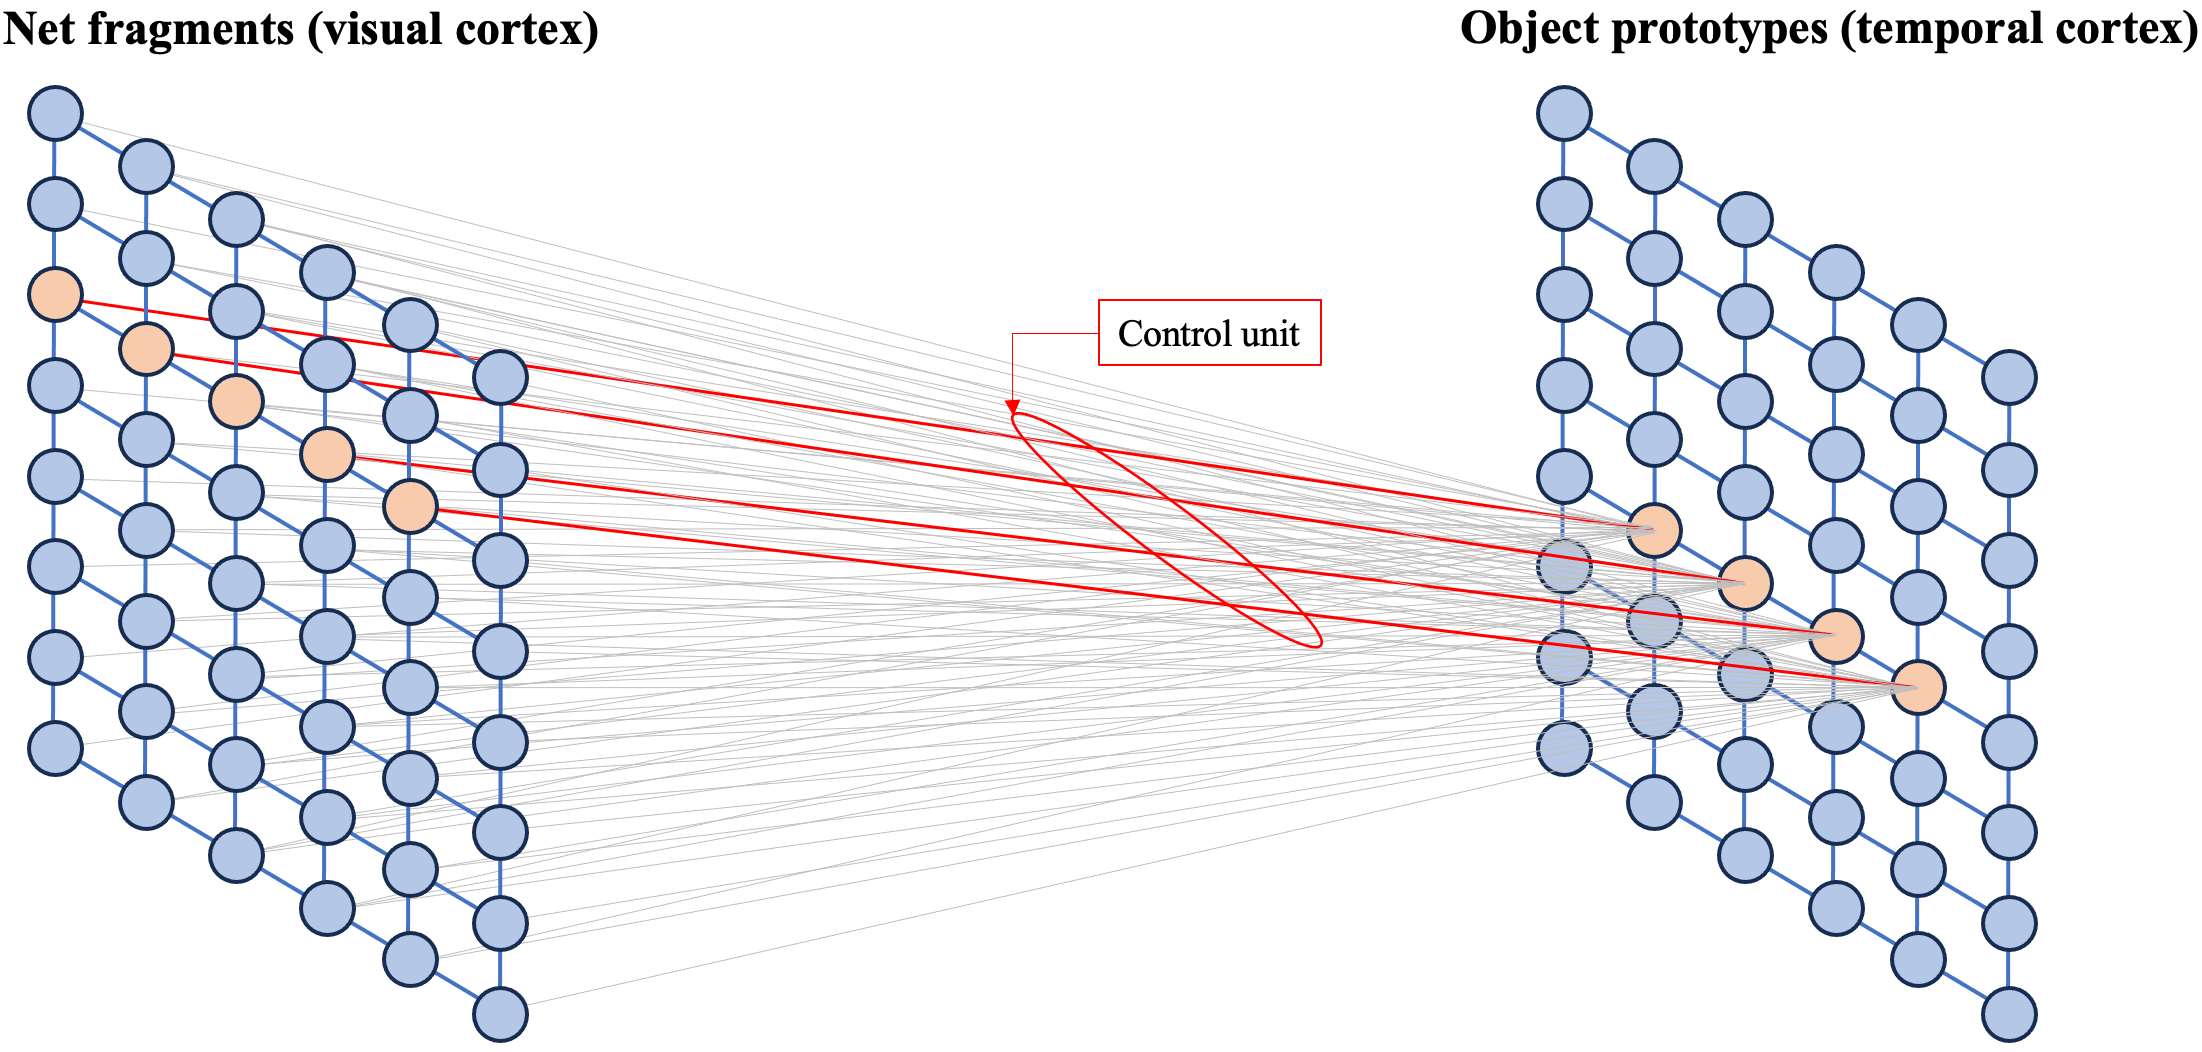
\includegraphics[width=0.99\textwidth]{maplets}
    \caption[An active maplet mapping net fragments to object prototypes]{Net fragments (on the left) are projected to an object (on the right). Many projection fibres (grey) run between the net fragments and objects, but only a few belonging to the same maplet (red) have been turned on.}
    \figlbl{maplets}
\end{figure}
%
As described at the beginning of this chapter, the visual cortex \sidecite{tong_primary_2003} extracts patterns from visual information \sidecite{grill-spector_human_2004}. This process is implemented with the aforementioned building blocks, such as lateral connections \sidecite{gilbert_lateral_1990, liang_interactions_2017, stettler_lateral_2002} and net fragments \cite{von_der_malsburg_concerning_2018}. In theory, this is sufficient to implement the principles from the Gestalt psychology \cite{ellis_source_1938, kohler_gestalt_1992, wagemans_century_2012, hamlyn_psychology_2017} and allows building feature hierarchies without early commitment \sidecite{marr_vision_2010}. However, it is not sufficient for efficient visual object detection.

In the human brain, object detection occurs in the temporal cortex \cite{miyashita_inferior_1993, conway_organization_2018}, a region spatially distant from the visual cortex.
The brain's solution to transmit information over such long distances are \emph{projection fibres} (a type of axons) \cite{tanigawa_organization_2005, greig_molecular_2013}.
Projection fibres are links between neurons in the visual cortex and object prototypes (so-called reference frames) in the temporal cortex \cite{goodale_separate_1992}.

Object prototypes in the temporal cortex are net fragments similar to those in the visual cortex. However, the visual cortex captures an overlay of fragments comprising cells activated by electrical pulses from the eyes.
This overlay of fragments describes a captured visual scene \cite{von_der_malsburg_theory_2022}, whereby it is unclear which sub-fragments represent distinct objects and how they are related.
On the other hand, the fragments in the temporal cortex depict one object, whereby these objects are position and transformation-invariant.

Projection fibres map neurons within the captured scene (in the primary visual cortex) to object prototypes (in the temporal cortex) with one-to-one connections \sidecite{anderson_shifter_1987}, where pairs of neurons connected in the visual cortex project to pairs of neurons connected in the temporal cortex topologically. The projection fibres have some flexibility, allowing for local distortions and enabling transformation- and position-invariant mapping \sidecite{wiskott_face_1996, wolfrum_recurrent_2008}. This mapping allows the recognition of one or more objects within a scene and their relationships to each other, facilitating object recognition and scene interpretation.

\subsubsection{Maplets and Control Units}
The ventral stream \sidecite{goodale_separate_1992} connects feature cells in the visual cortex to cells representing different object prototypes in the temporal cortex.  
Consequently, there is a multitude of projection fibres \sidecite{greig_molecular_2013, tanigawa_organization_2005}, but only a fraction are active at any given time \sidecite{anderson_shifter_1987, olshausen_neurobiological_1993}.
Typically, the same set of projection fibres is activated by similar patterns.
Such sets of projection fibres that are frequently activated simultaneously are grouped into \emph{maplets} \sidecite{zhu_maplets_2004}.
\emph{Control units} decide which maplets are activated and thus initiate the mapping between the visual and temporal cortex \cite{zhu_maplets_2004}. 
A control unit in the human brain is a unipolar neuron, a kind of neuron with extensions (so-called processes) that end in synapses and can conduct signals in both directions - from the synapse to the neuron and from the neuron to the synapse \sidecite{byrne_oxford_2019}.
Control units trigger a mapping when a net fragment in the visual cortex matches another fragment in the temporal cortex, i.e. when these two fragments have a high correlation \cite{zhu_maplets_2004}. However, they only remain active if numerous other projection fibres confirm the decision and map their respective fragments in the visual cortex to the same object prototype in a topological manner \sidecite{von_der_malsburg_concerning_2018}. By doing so, the human brain generates numerous hypotheses about observations, but inhibitory signals quickly deactivate most projections, leaving only the plausible ones active.

\figref{maplets} visualises such a projection between net fragments and an object prototype of a line. A vast amount of projection fibres (grey) run between these two areas, but only the most suitable ones are activated by the control unit of a maplet (red).
Please note that the line on the left is translated and stretched. Nevertheless, projection fibres still map such a transformed object to an idealised prototype.
\figref{maplets} shows a direct mapping from net fragments to prototypes for better clarity. In contrast, the mapping in the brain is done over several hierarchical levels, saving many projection fibres \sidecite{anderson_shifter_1987}.

Projection fibres thus provide generalisation, i.e. different, transformed versions of an object are recognised and mapped to a reference frame. This explains the ability of humans to see a new object once and immediately recognise it in a transformed version.

\subsection{Dynamic Mapping}\seclbl{neuroscience_findings_correspondence_finding}
Neuroscientific findings suggest that net fragments \sidecite{von_der_malsburg_theory_2022, von_der_malsburg_concerning_2018} are present in the visual and temporal cortex and that projection fibres map corresponding fragments topologically to implement object recognition \sidecite{greig_molecular_2013, liang_interactions_2017, stettler_lateral_2002}.
Further experiments demonstrate that the recognition time for humans depends on the size \sidecite{bundesen_visual_1975} and orientation \sidecite{jolicoeur_time_1985, lawson_effect_1999} of objects. Thus, it takes time to align the external world with internal representations.
This suggests that the brain implements an active dynamic process for correspondence finding rather than having a single forward pass.
Furthermore, physiological evidence exists that connections in the visual system are not static and suggest that receptive fields in the visual system change from one instance to the next to route the current neuronal activations to representations \sidecite{kusunoki_time_2003, womelsdorf_dynamic_2006}.
These findings suggest that projection fibres self-organise within a short time interval to initiate the corresponding mapping.


\subsection{Local Learning Principle}\seclbl{neuroscience_findings_local_learning_principle}
In the brain, consistency is evaluated at the level of individual synapses between each connected cell-pair \sidecite{hebb_organization_1949}. Each synapse is established if the firing of its source neuron and its target neuron are consistent, allowing the source neuron to predict the activity of the target neuron. This process is crucial for establishing net structures, where each neuron within a net fragment can predict the firing of other neurons with a high probability \sidecite{widrow_natures_2019}.

Such consistency is built between cells within the same layer connected by lateral connections \sidecite{stettler_lateral_2002} and between cells in different brain regions connected by projection fibres \cite{greig_molecular_2013, liang_interactions_2017}.
Building consistency means that the cells reach a consensus on what they represent \cite{von_der_malsburg_theory_2022}: Features trigger cells belonging to specific net fragments and only remain active if other laterally connected cells contribute to the same fragment and provide mutual support \sidecite{vogels_inhibitory_2011}. Cells that do not receive sufficient support are deactivated by inhibition \sidecite{coombs_specific_1955}.
Thus, cells agree on which net fragments (which features) are present in the input in a self-organising manner.
Consistency is achieved similarly between cells connected through projection fibres: Initially, many hypotheses (mappings) are activated, but after increasing inhibition, only the mapping receiving the most cell support remains active \cite{vogels_inhibitory_2011, von_der_malsburg_theory_2022}.
Thus, every active cell votes for net fragments and either remains active or is deactivated by inhibition until the entire network becomes consistent by agreeing on what features and objects are observed in the input \cite{von_der_malsburg_concerning_2018, von_der_malsburg_theory_2022}.

This local learning is a key difference between natural (animal or human) learning and the frequently used backpropagation of error \cite{rosenblatt_principles_1962, linnainmaa_taylor_1976}. With backpropagation, consistency is optimised at a single point \cite{crick_recent_1989, wang_comprehensive_2022}, specifically between the system's output and a teacher signal. All synapses, including those that are distantly connected (the ``deep'' connections), are guided by the consistency of this single point. Therefore, the human brain is dominated by local learning and self-organisation, while deep networks typically use a global learning rule that guides the learning process of the entire network.
While global learning works exceptionally well on specific tasks \cite{bertolini_machine_2021}, it completely fails to generalise between tasks and data domains compared to humans.

\section{Long-Term Vision}\seclbl{biologial_inspiration_vision}
The aforementioned neuroscientific findings serve as the foundation for building a novel image-processing framework.
The core behind this framework is based on two stages (representing the primary visual \sidecite{tong_primary_2003, grill-spector_human_2004} and temporal cortex \sidecite{miyashita_inferior_1993, conway_organization_2018}) and projection fibres connecting them \sidecite{greig_molecular_2013, tanigawa_organization_2005}.
The first stage builds net fragments \sidecite{von_der_malsburg_concerning_2018} using lateral connections \sidecite{gilbert_lateral_1990, liang_interactions_2017, stettler_lateral_2002}, reassembling a visual scene captured with a sensory system (the eyes).
The second stage contains reference frames representing specific objects. These objects are centred and transformation-invariant and can thus afford longer-reaching lateral connections.
Multiple 2D reference frames must exist for each object to represent an object from various viewpoints.
Projection fibres connect these two stages \cite{tanigawa_organization_2005, greig_molecular_2013}, mapping objects within a visual scene to object prototypes.
This mapping serves as a scene interpretation layer by describing which objects are located where in the observed scene.
In \chref{probabilistic_framework}, a framework is proposed that implements these two stages linked with projection fibres.
It is considered a computational implementation of the fundamentals of the biological visual system.
However, in the long term, this framework can be further extended and is not limited to these two stages, enabling highly efficient scene processing.
These extensions are discussed in the following.

\subsection{Object Classification}
A classification layer maps an object to a specific instance \sidecite{schmarje_survey_2021}, for example, a person, to a person's name. Projection fibres do not provide such a classification as these fibres map the pattern to a more generalised view, i.e. transforming a person to a reference person. Instead, a subsequent memory stage (related to the brain's inferior cortex \sidecite{miyashita_inferior_1993}) is needed to map a reference object to an actual label.
This memory stage contains multiple instances for each object and provides distinction between objects. The memory stage implements an $n$-to-$n$ mapping to the reference frame: Each reference frame has multiple instances (e.g. multiple persons exist), and each instance can belong to multiple reference frames (e.g. a face and a body could be different reference frames but belong to the same instance).

The human brain has single cells representing specific instances of objects \sidecite{gross_genealogy_2002}.
Therefore, memory is assumed to consist of one or a few cells representing a ``label'', while reference frames consist of many cells describing an object's appearance \cite{von_der_malsburg_concerning_2018, von_der_malsburg_theory_2022}.
This allows storing and distinguishing many object instances while not requiring a vast number of cells.


\subsection{Scene Interpretation}
Projection fibres map all objects within an observed scene to prototypes. Thus, the projection fibres implement object segmentation and identification.
In addition, the position of each object is known, as well as the relative differences in position between the objects.
Such a mapping provides a mental description of a perceived scene and answers the question of which object is where. However, having a description is not sufficient to interpret a scene. For scene interpretation, all objects must be put into context.

As described in \secref{neuroscience_findings_local_learning_principle}, consistency is built between the cells within the two stages to build net fragments and between the projection fibres connecting net fragments \sidecite{von_der_malsburg_theory_2022, liang_interactions_2017, stettler_lateral_2002}.
In the long term, more components must be added, allowing to build consistency between memories and reference frames as well.
For instance, projection fibres could map one object in the scene to a person while mapping another object in close spatial proximity of this person's foot to a ball. By building consistency between these two objects, one could conclude that this person is most likely playing football (soccer). Synaptic connections between these references could be formed if such scenes are observed several times, allowing for scene interpretation.
Thus, observing people touching a ball with their feet corresponds to a pattern the system frequently observes, characterised by the simultaneous activity of the corresponding net fragments and their relative position. By integrating this activity with relative positions and applying Hebbian updates, the network learns this pattern corresponding to football. 
After the pattern has been learned, cells can vote for it by providing lateral support to this scene interpretation, and the consistency property describes if an observed scene corresponds to playing football or not.
Furthermore, memories \sidecite{liu_optogenetic_2012, miyashita_inferior_1993} could be integrated to confirm or reject this hypothesis. If, for example, the person is identified as a soccer player such as Ronaldo, it would further strengthen this hypothesis.

A system building consistency between object prototypes, relative object positions, and memories could learn interpretations of visual scenes and might have the potential to ``understand'' how objects are related to each other. A pivotal difference to deep networks is that the model can build such consistency on its own, while deep learning systems require a teaching signal to learn consistency.
I speculate that having a system that can build consistency of completely unseen scenes without teaching signals might be an important step towards emergence.


\subsection{Avoiding Early Commitment}\seclbl{biologial_inspiration_early_commitment}
As described in the \secref{intro_motivation}, deep learning models are prone to early commitment \sidecite{marr_vision_2010}.
The brain's solution to prevent early commitment is building net fragments.
A single layer with lateral connections that forms net fragments can represent local and global features at the same time\sidenote{This way of thinking about features can be hard to comprehend, especially for computer scientists familiar with deep learning.}.
Each set of active and laterally connected neurons can be considered a net fragment. Net fragments with few cells depict local features, while fragments containing many features represent global features.

A system that avoids the fallacy of early commitment should solve the conundrum that local decisions are taken based on plausibility in the light of high-level patterns, while high-level patterns can only be defined based on low-level features.
The most fundamental local decision is whether a single cell should be active. Since a single cell receives support from all laterally connected cells, a high-level pattern (i.e. the activity of all directly or indirectly connected cells) is used to make this decision. Therefore, local decisions are taken based on high-level patterns. The high-level pattern used to make this decision is defined by the sum of individual cells (i.e. low-level features). Hence, the human brain solves the conundrum within every single layer.


\subsubsection{Hierarchical Features}
Neuroscientific findings indicate that the human brain does not rely on a sequence of layers to build feature hierarchies as typically done in deep networks \sidecite{prince_understanding_2023}.
In the biological context, layers have other connotations, and evidence suggests that layers in cortical columns deal with depth rotations \sidecite{iamshchinina_perceived_2021}.
In the proposed framework, feature hierarchies are implicitly stored in net fragments whereby a larger fragment represents a global feature, and smaller fragments represent local features.
Consequently, sequences of layers are not necessary to represent feature hierarchies.

However, multiple stages are required to build abstractions of input signals, i.e. to generalise features.
In the human brain, several regions interact to generate abstractions \sidecite{felleman_distributed_1991}.
In fact, the visual cortex builds net fragments based on signals from the eyes, projection fibres map the object to prototypes, and other fibres map the prototypes to memories and interpret them. Thus, various stages are involved in processing images.
Furthermore, processing occurs quickly until all stages reach a consensus \sidecite{fernandes_self-organization_2015}. Thus, no layer-wise processing is required as in deep learning, but multiple stages interact with each other to build feature abstractions. As described in \secref{neuroscience_findings_correspondence_finding}, these interactions are a dynamic, iterative process rather than a single forward pass.

